

\section{Numerical Experiments} \label{sec:res}

\subsection{Vortex Merging}
Consider the $2D$ incompressible Euler equation, \eqref{eq:3.8} with no viscous term, on a square domain $\Omega = [0,2\pi]^2$, provided with periodic boundary conditions. Spatial derivatives are discretized using a Fourier spectral method, which in centered differential operators in the Fourier space. To capture the fine details characterizing the solution, $256\times 256$ modes have been adopted. The initial condition is given in terms of the vorticity distribution $\mathbf{\omega} = \nabla \times u$ {\commnet \{ check this \}}. 

We consider the evolution of three different vortices, and the initial structure is given by
\begin{equation}\label{eqn:initial_cond_vort}
\omega = \omega_0 + \sum_{i=1}^{3} \alpha_i e^{-\dfrac{\left(x-x_i\right)^{2}+\left(y-y_i\right)^{2}}{\beta^2}}.
\end{equation}
In \eqref{eqn:initial_cond_vort}, $(x,y)$ represents the spatial coordinates, $\left( x_i, y_i\right)$ is the center of the $i$th vortex, $\alpha_i$ its maximum amplitude, and $\beta$ controls the effective radius of the vortex. In this example, the center of three vortices are positioned at 
\begin{equation}
\left( x_1, y_1 \right) = \left(0.75\pi,\pi\right) , \left( x_2, y_2 \right) = \left(1.25\pi,\pi\right), \left( x_3, y_3 \right) = \left(1.25\pi,1.5\pi\right),
\end{equation}
close to the center of the domain, of which, two have positive spins with $\alpha_1 = \alpha_2 = \pi$ and the other rotates in the opposite direction with $\alpha_3 = -0.5\pi$. The effective radius of all the vortices is set to $\beta = 1 / \pi$. This arrangement of vortices is an effective initial condition for the process of merging vortices. This phenomenon is often a result of fast-moving dipoles {\commnet \{ what is a dipole?\}} facing another vortex {\commnet \{ ref \}}. The forces developed in the merging process transfers the vorticity from the initial configuration, into long, narrow, and spiral-shaped strips of intense vorticity \cite{filaments_vort}. The formation of such thin vorticity filaments in the fluid, can pose numerical challenges. 

In the context of MOR, conservation of energy and stability is crucial for capturing fined structures, mentioned above. In the absence of natural dissipation, characterizing the Euler equation, straight forward application of MOR techniques is often unstable.

To define the initial conditions in terms of the velocity components $\omega$ and the pressure $p$, we define a stream-function $\Psi$, the solution to the equation 
\begin{equation} \label{eq:5.1}
	\nabla \Psi = \omega.
\end{equation}
The initial velocity is then given by $\nabla \times \Psi$. To solve the stream-function problem \eqref{eq:5.1}, we require $\int_{\Omega} \omega \ dx= 0$ {\commnet \{ check this \}}. It is easily verified that this requirement implies $\omega_0 = 0.038$. The pressure is recovered by solving the related Poisson pressure equation {\commnet \{ write the equation here \}}. The implicit midpoint scheme, to mimic the time integration scheme presented in \eqref{eq:3.27}, is considered to integrate in time. The merging phenomenon is simulated for a total of $18$ time units using a temporal step $\Delta t=0.004$.

\Cref{fig:unstable_full_models} illustrates the evolution of the kinetic energy for the advective, divergence, and the skew-symmetric form of the high-fidelity system. It is observed that only the skew-symmetric form preserves the kinetic energy, confirming the results in \Cref{sec:skew.2}.

%%%%%%%%%%%%%%%%%%%%%%%%%%%%%%%%%%%%%%%%%
%%%%% Comparison Skew symmetric, divergence and advective form %%%%%
%%%%%%%%%%%%%%%%%%%%%%%%%%%%%%%%%%%%%%%%%
\begin{figure}[t]
  \centering
  \begin{tikzpicture}[scale=0.5452]
    \begin{axis}[ylabel=$E_K(t)$,
                 xlabel=$t$,
                 label style={font=\large},
                 legend pos=south west,
                 legend entries={Skew Symmetric form, Divergent form, Advective form},
                 legend style={font=\large},
                 width=0.7\linewidth, 
                 height=0.5\linewidth,
                 minor x tick num=1,
                 minor y tick num=2,	
                 yticklabel style={/pgf/number format/.cd,fixed,precision=4},
                 scaled x ticks = true,
                 enlargelimits=false,
                 scale only axis]
                 \addplot[color=red,style=solid,style=ultra thick]  table[x = time, y = energy] {./data/Incompressible_Euler/Energy_compare_formulations/energy_skew_symmetric.txt};
                 \addplot[color=blue,style=solid,style=ultra thick]  table[x = time, y = energy] {./data/Incompressible_Euler/Energy_compare_formulations/energy_divergence.txt};
                 \addplot[color=black!50!green,style=solid,style=ultra thick]  table[x = time, y = energy] {./data/Incompressible_Euler/Energy_compare_formulations/energy_convective.txt};
    \end{axis}%  
  \end{tikzpicture}
  \caption{Conservation of the kinetic energy $K$ for the advective, divergence and the skew-symmetric formulations. {\commnet \{ please change Divergent to Divergence in the legend \}} }
  \label{fig:unstable_full_models}
\end{figure}
A total of $5000$ temporal snapshots is used to construct a reduced basis, following the process discussed in \Cref{sec:mor}. The decay of the singular values, as an indication of the reducibility of the problem, is presented in \Cref{fig:RIC}. The first $35$ POD modes corresponds to over $99\%$ of the {\commnet \{ kinetic? \}} energy of the high fidelity solution. This suggests that an accurate reduced system can be constructed using a small number of basis vectors. To illustrate the effectiveness of the method, smaller bases are also considered.

For a qualitative analysis, in Figure \ref{fig:snap_solution_incompressible_Euler}, four snapshots at different time frames are shown for the high fidelity system and reduced system with $k=17$ and $k=35$ modes. It is seen that the overall dynamics of the problem, and in particular the formation and development of vorticity filaments, are correctly represented, even with a moderate number of basis vectors. Although small details are not captured by the reduced system with a small number of basis vectors, the position and the spreading of the vortices are comparable. 

%%%%%%%%%%%%%%%%%%%%%%%%%%%%%%%%%%%%%%%%%%%%
%%%%%%%%%%%%%% Snapshots of merging process %%%%%%%%%%%%%%
%%%%%%%%%%%%%%%%%%%%%%%%%%%%%%%%%%%%%%%%%%%%
\begin{figure}[t]
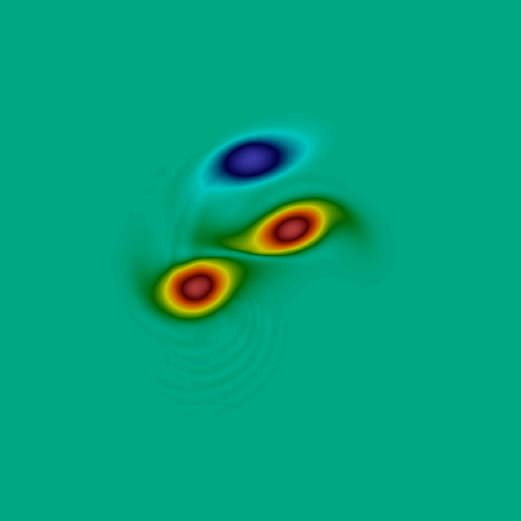
\includegraphics[scale=0.06]{data/Incompressible_Euler/Snapshots/red_17_2.png}\hspace{1em}
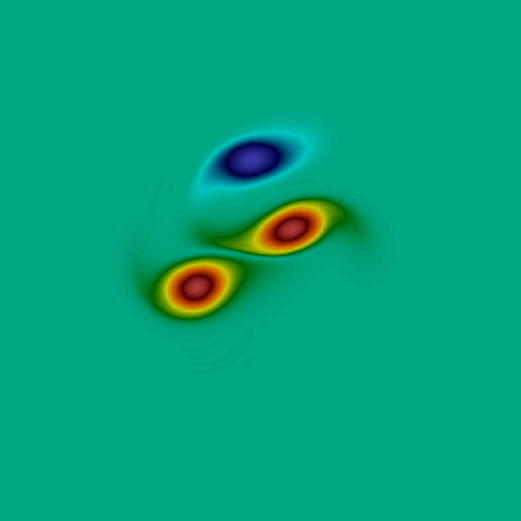
\includegraphics[scale=0.06]{data/Incompressible_Euler/Snapshots/red_35_2.png}\hspace{1em}
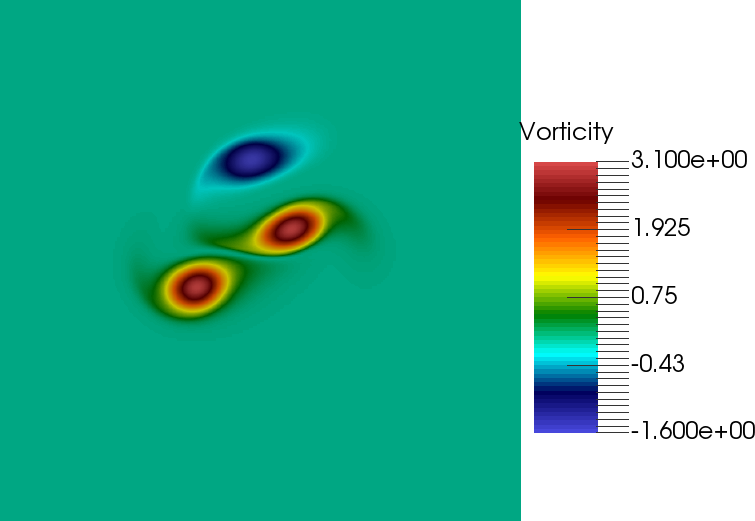
\includegraphics[scale=0.06]{data/Incompressible_Euler/Snapshots/Full_2.png}\\

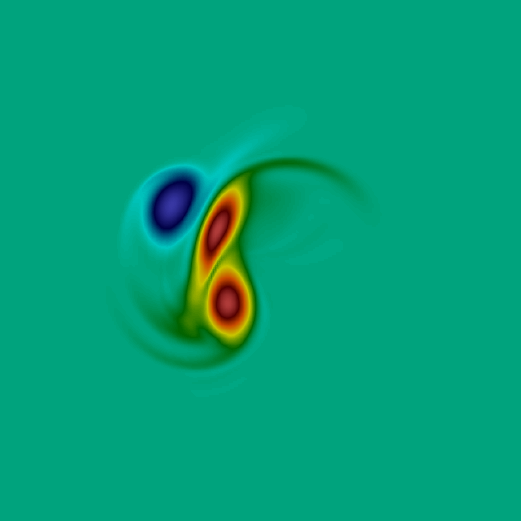
\includegraphics[scale=0.06]{data/Incompressible_Euler/Snapshots/red_17_3.png}\hspace{1em}
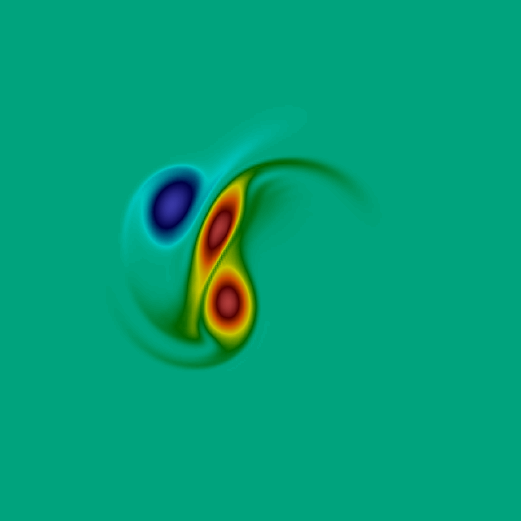
\includegraphics[scale=0.06]{data/Incompressible_Euler/Snapshots/red_35_3.png}\hspace{1em}
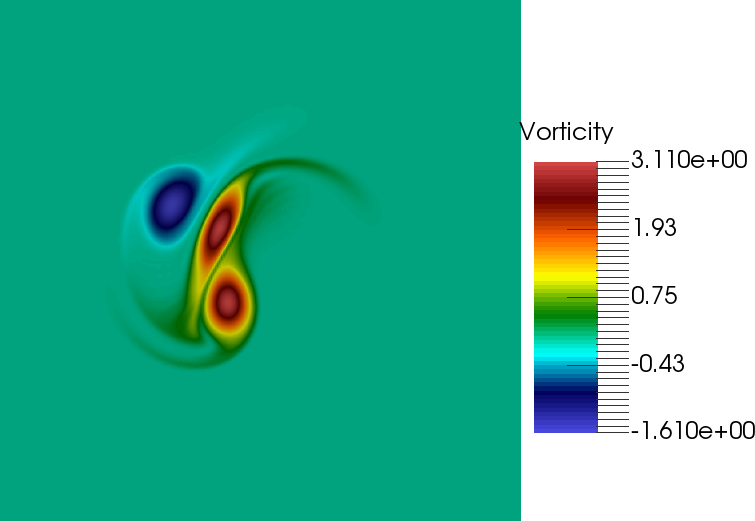
\includegraphics[scale=0.06]{data/Incompressible_Euler/Snapshots/Full_3.png}\\

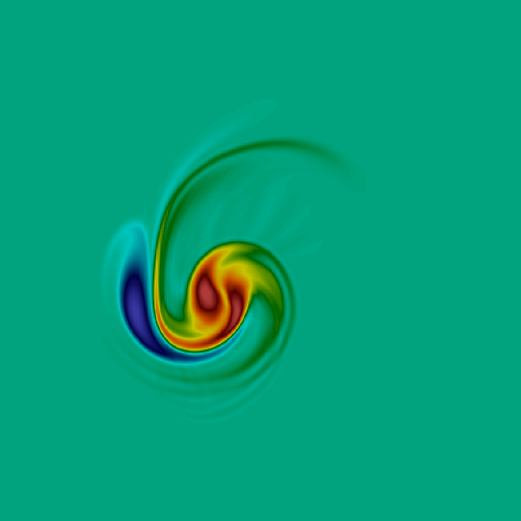
\includegraphics[scale=0.06]{data/Incompressible_Euler/Snapshots/red_17_4.png}\hspace{1em}
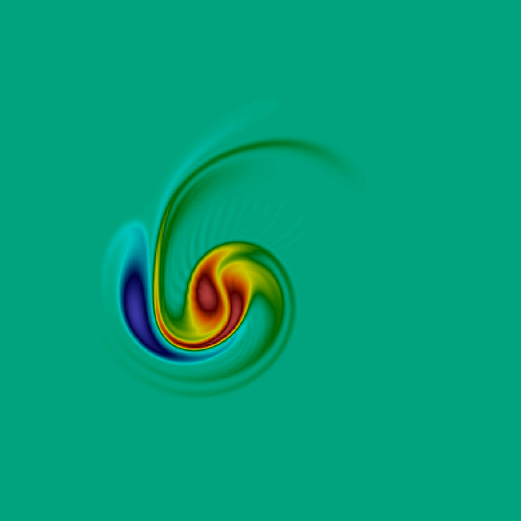
\includegraphics[scale=0.06]{data/Incompressible_Euler/Snapshots/red_35_4.png}\hspace{1em}
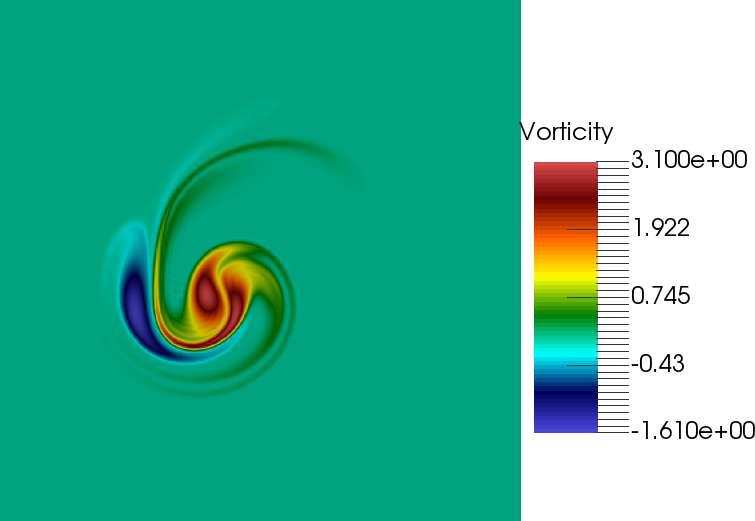
\includegraphics[scale=0.06]{data/Incompressible_Euler/Snapshots/Full_4.png}\\

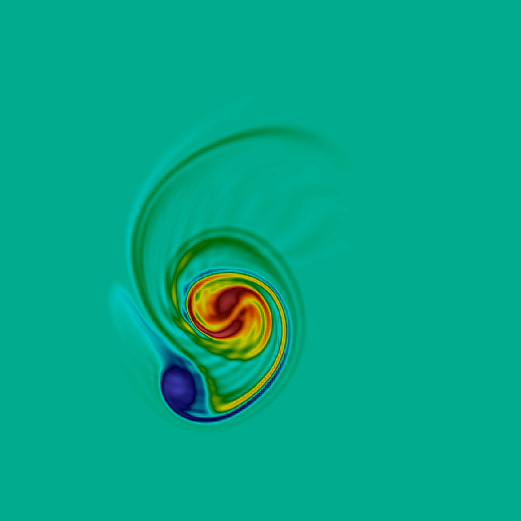
\includegraphics[scale=0.06]{data/Incompressible_Euler/Snapshots/red_17_5.png}\hspace{1em}
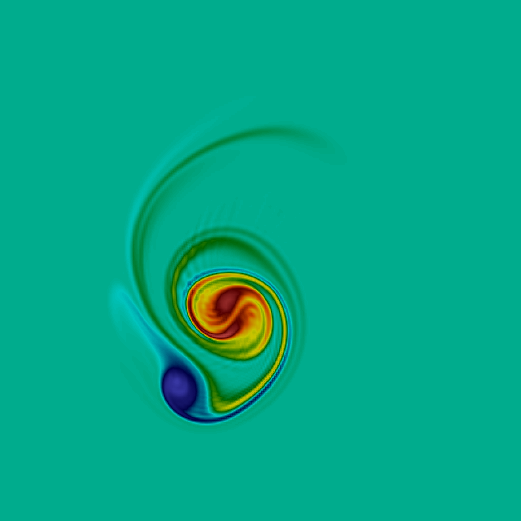
\includegraphics[scale=0.06]{data/Incompressible_Euler/Snapshots/red_35_5.png}\hspace{1em}
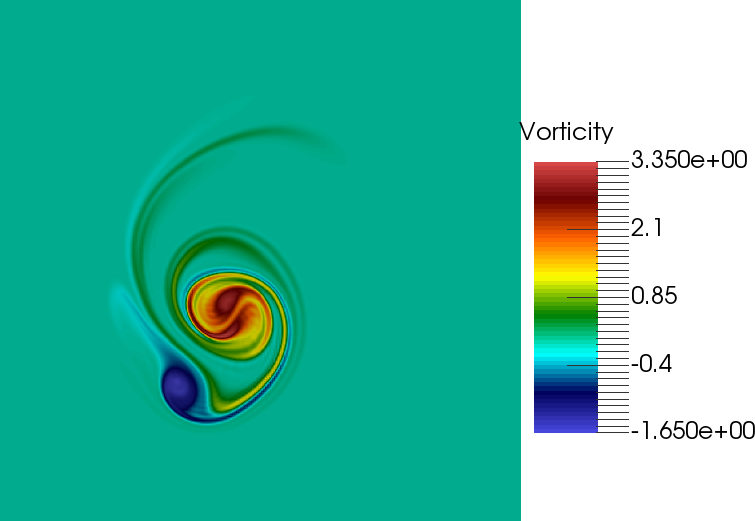
\includegraphics[scale=0.06]{data/Incompressible_Euler/Snapshots/Full_5.png}

\caption{Snapshots of the high-fidelity system and the reduced system at $t=\left\{ 4,8,12,18 \right\}$. From left to right: the snapshots of the reduced model with $k=17$, $k=35$ and the high fidelity solution.}
\label{fig:snap_solution_incompressible_Euler}
\end{figure}


%%%%%%%%%%%%%%%%%%%%%%%%%%%%%%%%%%%%%%%%%%
%%%%%%%%%% Singular values decay merging vorteces %%%%%%%%%%%
%%%%%%%%%%%%%%%%%%%%%%%%%%%%%%%%%%%%%%%%%%
\begin{figure}[t]
\centering
\begin{tikzpicture}[scale=0.5452]
    \begin{semilogyaxis}[ylabel = $\frac{\sigma_j}{\sum_i \sigma_i}$,
                 xlabel=Basis ,
                 label style={font=\large},
                 %legend pos=north east,
                 %legend entries={$k=24$ Div,$k=102$ Div,$k=201$ Div,$k=24$ Skew,$k=102$ Skew,$k=201$ Skew},
                 legend style={font=\large},
                 grid=both,
                 ticks=both,
                 width=0.7\linewidth, 
                 height=0.5\linewidth,
                 minor x tick num=1,
                 minor y tick num=2,	
                 yticklabel style={/pgf/number format/.cd,fixed,precision=9},
                 scaled x ticks = true,
                 enlargelimits=false,
                 scale only axis,
                 ymin=0,
                 ymax = 2,
                 samples = 100]
                 \addplot[color=black,style=solid,style=ultra thick]  table[x = x, y = s] {./data/Incompressible_Euler/Singular_values/sv.txt};
    \end{semilogyaxis}
\end{tikzpicture}
\caption{The decay of the singular values for the merging vortices problem. {\commnet \{please put this figure and figure 1 into a single figure (Left and right to each other)\} } }
\label{fig:RIC}
\end{figure}
\Cref{fig:approx_error_incompressible_Euler} shows the 2-norm error between the high-fidelity solution and the approximated solution. It is seen that the error decreases, consistently, as the number of basis vectors increase. Furthermore, the accuracy is maintained over the period of time integration.

The conservation of the kinetic energy is presented in \Cref{fig:energy_error_incompressible_Euler}. It is seen that even for a small number of basis vectors, where the solution is not well approximated, the kinetic energy is conserved. Furthermore, it is observed that the error in the kinetic energy, due to MOR, is constant in time. This helps with the robustness of the reduced system over long time-integration.


%%%%%%%%%%%%%%%%%%%%%%%%%%%%%%%%%%%%%%%%%%%
%%%%%%%%%% Approximation error and energy conservation %%%%%%%%%%
%%%%%%%%%%%%%%%%%%%%%%%%%%%%%%%%%%%%%%%%%%%
\begin{figure}[t]
\centering
\begin{subfigure}[]{0.47\linewidth}
\begin{tikzpicture}[scale=0.58]
    \begin{semilogyaxis}[ylabel = $\left | \mathbf{v}(t)-\mathbf{v}^r(t) \right |^2$,
                 xlabel=$t$,
                 label style={font=\large},
                 legend style={font=\large},
                 grid=both,
                 ticks=both,
                 width=1.4\linewidth, 
                 height=1.0\linewidth,
                 minor x tick num=1,
                 minor y tick num=2,	
                 yticklabel style={/pgf/number format/.cd,fixed,precision=9},
                 scaled x ticks = true,
                 enlargelimits=false,
                 scale only axis,
                 samples = 100,
                 cycle list name=exotic]
                 \addplot+[style=solid,style=ultra thick]  table[x = time, y = error] {./data/Incompressible_Euler/Approximation_Error/err_5.txt};
                 \addplot+[style=solid,style=ultra thick]  table[x = time, y = error] {./data/Incompressible_Euler/Approximation_Error/err_8.txt};
                 \addplot+[style=solid,style=ultra thick]  table[x = time, y = error] {./data/Incompressible_Euler/Approximation_Error/err_11.txt};
                 \addplot+[style=solid,style=ultra thick]  table[x = time, y = error] {./data/Incompressible_Euler/Approximation_Error/err_14.txt};
                 \addplot+[style=solid,style=ultra thick]  table[x = time, y = error] {./data/Incompressible_Euler/Approximation_Error/err_23.txt};
                 \addplot+[style=solid,style=ultra thick]  table[x = time, y = error] {./data/Incompressible_Euler/Approximation_Error/err_26.txt};
                 \addplot+[style=solid,style=ultra thick]  table[x = time, y = error] {./data/Incompressible_Euler/Approximation_Error/err_29.txt};
                 \addplot+[style=solid,style=ultra thick]  table[x = time, y = error] {./data/Incompressible_Euler/Approximation_Error/err_35.txt};
    \end{semilogyaxis}
\end{tikzpicture}
\caption{}
\label{fig:approx_error_incompressible_Euler}
\end{subfigure} \hfill
\begin{subfigure}[]{0.47\linewidth}
\begin{tikzpicture}[scale=0.58]
    \begin{axis}[ylabel = $|K(t)-K_r^{r}(t)|$,
                 xlabel=$t$,
                 label style={font=\large},
                 legend pos=south west,
                 legend entries={$k=5$ , $k=8$, $k=11$, $k=14$, $k=23$, $k=26$, $k=29$, $k=35$},
                 legend style={font=\large},
                 grid=both,
                 ticks=both,
                 width=1.4\linewidth, 
                 height=1.0\linewidth,
                 minor x tick num=1,
                 minor y tick num=2,	
                 yticklabel style={/pgf/number format/.cd,fixed,precision=9},
                 scaled x ticks = true,
                 enlargelimits=false,
                 scale only axis,
                 ymax = 0.5598,
                 samples = 100,
                 cycle list name=exotic]
                 \addplot+[style=solid,style=ultra thick]  table[x = time, y = error] {./data/Incompressible_Euler/Energy_conservation/ene_full_5.txt};
                 \addplot+[style=solid,style=ultra thick]  table[x = time, y = error] {./data/Incompressible_Euler/Energy_conservation/ene_full_8.txt};
                 \addplot+[style=solid,style=ultra thick]  table[x = time, y = error] {./data/Incompressible_Euler/Energy_conservation/ene_full_11.txt};
                 \addplot+[style=solid,style=ultra thick]  table[x = time, y = error] {./data/Incompressible_Euler/Energy_conservation/ene_full_14.txt};
                 \addplot+[style=solid,style=ultra thick]  table[x = time, y = error] {./data/Incompressible_Euler/Energy_conservation/ene_full_23.txt};
                 \addplot+[style=solid,style=ultra thick]  table[x = time, y = error] {./data/Incompressible_Euler/Energy_conservation/ene_full_26.txt};
                 \addplot+[style=solid,style=ultra thick]  table[x = time, y = error] {./data/Incompressible_Euler/Energy_conservation/ene_full_29.txt};
                 \addplot+[style=solid,style=ultra thick]  table[x = time, y = error] {./data/Incompressible_Euler/Energy_conservation/ene_full_35.txt};
    \end{axis}
\end{tikzpicture}
\caption{}
\label{fig:energy_error_incompressible_Euler}
\end{subfigure}
\label{fig:energy_approx_err}
\caption{(\protect\subref{fig:approx_error_incompressible_Euler}) Evolution of 2-norm error in velocity, between the high-fidelity system and the reduced system. (\protect\subref{fig:energy_error_incompressible_Euler}) Conservation of the kinetic energy. {\commnet \{ in fig a $y$ axis: $\| u - \tilde u \|_2$ \} \{ in fig b $|k - \tilde K|$ \}}  }
\end{figure}


\subsection{The Compressible Euler Equation}
\subsubsection{2D Kelvin-Helmholtz instability}
%%%%%%%%%%%%%%%%%%%%%%%%%%%%%%%%%%%%%%%%%%%%
%%%%%%%%%%%%%%%% Approximation Error %%%%%%%%%%%%%%%%%
%%%%%%%%%%%%%%%%%%%%%%%%%%%%%%%%%%%%%%%%%%%%
\begin{figure}
\centering
\begin{subfigure}[]{0.48\linewidth}
  \begin{tikzpicture}[scale=0.55]
    \begin{semilogyaxis}[xlabel=$t$,
                 ylabel=$e(t)$,
                 label style={font=\large},
                 legend pos=outer north east,
                 legend style={font=\large},
                 legend entries={$k=200$,$k=300$,$k=400$,$k=500$,$k=600$},
                 grid=both,
                 ticks=both,
                 width=1.4\linewidth, 
                 height=1.0\linewidth,
                 minor x tick num=1,
                 minor y tick num=2,	
                 yticklabel style={/pgf/number format/.cd,fixed,precision=9},
                 scaled x ticks = true,
                 enlargelimits=false,
                 scale only axis,
                 cycle list name=exotic]
                 \addplot+[style=solid,style=ultra thick]  table[x = time, y = quantity] {./data/Compressible_Euler/KH/error/error_200.txt};  
                 \addplot+[style=solid,style=ultra thick]  table[x = time, y = quantity] {./data/Compressible_Euler/KH/error/error_300.txt};      
                 \addplot+[style=solid,style=ultra thick]  table[x = time, y = quantity] {./data/Compressible_Euler/KH/error/error_400.txt}; 
                 \addplot+[style=solid,style=ultra thick]  table[x = time, y = quantity] {./data/Compressible_Euler/KH/error/error_500.txt};      
                 \addplot+[style=solid,style=ultra thick]  table[x = time, y = quantity] {./data/Compressible_Euler/KH/error/error_600.txt};               
    \end{semilogyaxis}%  
  \end{tikzpicture}
\end{subfigure}
\caption{Evolution in time of the error  between the high fidelity solution of the Kelvin-Helmoltz and the reduced solution for different number of basis $k$. As error measure we consider $e(t)=\sqrt{\|\mathbf{r}-\mathbf{r}^r\|^2+\|\mathbf{u_xr}-\mathbf{u_xr}^r\|^2 + \|\mathbf{u_yr}-\mathbf{u_yr}^r\|^2 + \|\mathbf{p}-\mathbf{p}^r\|^2}$.}
\end{figure}

\begin{figure}
  \centering
  \begin{subfigure}[]{0.48\linewidth}
  \begin{tikzpicture}[scale=0.55]
    \begin{semilogyaxis}[ylabel = $\left|\mathbf{1}^T(\mathbf{r}-\mathbf{r}^r)(t)\right|$,
                 xlabel=$t$,
                 label style={font=\large},
                 legend pos=north east,
                 legend entries={$k=200$ ,$k=300$, $k=400$,$k=500$,$k=600$},
                 legend style={font=\large},
                 grid=both,
                 ticks=both,
                 width=1.4\linewidth, 
                 height=1.0\linewidth,
                 minor x tick num=1,
                 minor y tick num=2,	
                 %yticklabel style={/pgf/number format/.cd,fixed,precision=9},
                 scaled x ticks = true,
                 enlargelimits=false,
                 scale only axis,
                 cycle list name=exotic]
                 \addplot+[style=solid,style=ultra thick]  table[x = time, y = quantity] {./data/Compressible_Euler/KH/conserved_quantities/mass_red_200.txt};
                 \addplot+[style=solid,style=ultra thick]  table[x = time, y = quantity] {./data/Compressible_Euler/KH/conserved_quantities/mass_red_300.txt};
                 \addplot+[style=solid,style=ultra thick]  table[x = time, y = quantity] {./data/Compressible_Euler/KH/conserved_quantities/mass_red_400.txt};
                 \addplot+[style=solid,style=ultra thick]  table[x = time, y = quantity] {./data/Compressible_Euler/KH/conserved_quantities/mass_red_500.txt};
                 \addplot+[style=solid,style=ultra thick]  table[x = time, y = quantity] {./data/Compressible_Euler/KH/conserved_quantities/mass_red_600.txt};
    \end{semilogyaxis}%  
  \end{tikzpicture}
  \caption{}
  \label{mass_error_KH}
  \end{subfigure}\hfill
  \begin{subfigure}[]{0.48\linewidth}
  \begin{tikzpicture}[scale=0.55]
    \begin{semilogyaxis}[ylabel = $\left|(\mathbf{r}^{T}\mathbf{u}-\mathbf{r}^{rT}\mathbf{u}^{r})(t)\right|$,
                 xlabel=$t$,
                 label style={font=\large},
                 legend pos=north east,
%                 legend entries={$k=200$ Conv,$k=201$ Conv},
                 legend style={font=\large},
                 grid=both,
                 ticks=both,
                 width=1.4\linewidth, 
                 height=1.0\linewidth,
                 minor x tick num=1,
                 minor y tick num=2,	
                 %yticklabel style={/pgf/number format/.cd,fixed,precision=9},
                 scaled x ticks = true,
                 enlargelimits=false,
                 scale only axis,
                 cycle list name=exotic]
                 \addplot+[style=solid,style=ultra thick]  table[x = time, y = quantity] {./data/Compressible_Euler/KH/conserved_quantities/momentum_red_200.txt};
                 \addplot+[style=solid,style=ultra thick]  table[x = time, y = quantity] {./data/Compressible_Euler/KH/conserved_quantities/momentum_red_300.txt};
                 \addplot+[style=solid,style=ultra thick]  table[x = time, y = quantity] {./data/Compressible_Euler/KH/conserved_quantities/momentum_red_400.txt};
                 \addplot+[style=solid,style=ultra thick]  table[x = time, y = quantity] {./data/Compressible_Euler/KH/conserved_quantities/momentum_red_500.txt};
                 \addplot+[style=solid,style=ultra thick]  table[x = time, y = quantity] {./data/Compressible_Euler/KH/conserved_quantities/momentum_red_600.txt};
    \end{semilogyaxis}%  
  \end{tikzpicture}
  \caption{}
  \label{momentum_error_KH}
  \end{subfigure}
  
  \begin{subfigure}[]{0.48\linewidth}
  \begin{tikzpicture}[scale=0.55]
    \begin{semilogyaxis}[ylabel = $\left| \dfrac{1}{2}\left( \mathbf{u}^{rT}\mathbf{R}^r\mathbf{u}^r-\mathbf{u}^{T}\mathbf{R}\mathbf{u}\right)\right|$,
                 xlabel=$t$,
                 label style={font=\large},
                 legend pos=north east,
%                 legend entries={$k=200$ Conv,$k=201$ Conv},
                 legend style={font=\large},
                 grid=both,
                 ticks=both,
                 width=1.4\linewidth, 
                 height=1.0\linewidth,
                 minor x tick num=1,
                 minor y tick num=2,	
                 %yticklabel style={/pgf/number format/.cd,fixed,precision=9},
                 scaled x ticks = true,
                 enlargelimits=false,
                 scale only axis,
                 cycle list name=exotic]
                 \addplot+[style=solid,style=ultra thick]  table[x = time, y = quantity] {./data/Compressible_Euler/KH/conserved_quantities/energy_red_200.txt};
                 \addplot+[style=solid,style=ultra thick]  table[x = time, y = quantity] {./data/Compressible_Euler/KH/conserved_quantities/energy_red_300.txt};
                 \addplot+[style=solid,style=ultra thick]  table[x = time, y = quantity] {./data/Compressible_Euler/KH/conserved_quantities/energy_red_400.txt};
                 \addplot+[style=solid,style=ultra thick]  table[x = time, y = quantity] {./data/Compressible_Euler/KH/conserved_quantities/energy_red_500.txt};
                 \addplot+[style=solid,style=ultra thick]  table[x = time, y = quantity] {./data/Compressible_Euler/KH/conserved_quantities/energy_red_600.txt};
    \end{semilogyaxis}%  
  \end{tikzpicture}
   \caption{}
  \label{energy_error_KH}
  \end{subfigure}
\caption{Comparison between the high fidelity solution of the Kelvin-Helmholtz problem and the reduced solution of the mass (\protect\subref{mass_error_KH}), the momentum (\protect\subref{momentum_error_KH}), and the total energy (\protect\subref{energy_error_KH}).}
\end{figure}

%%%%%%%%%%%%%%%%%%%%%%%%%%%%%%%%%%%%%
%%%%%%%%%%%%%% Snapshots of KH %%%%%%%%%%%%%%
%%%%%%%%%%%%%%%%%%%%%%%%%%%%%%%%%%%%%
\begin{figure}[h!]
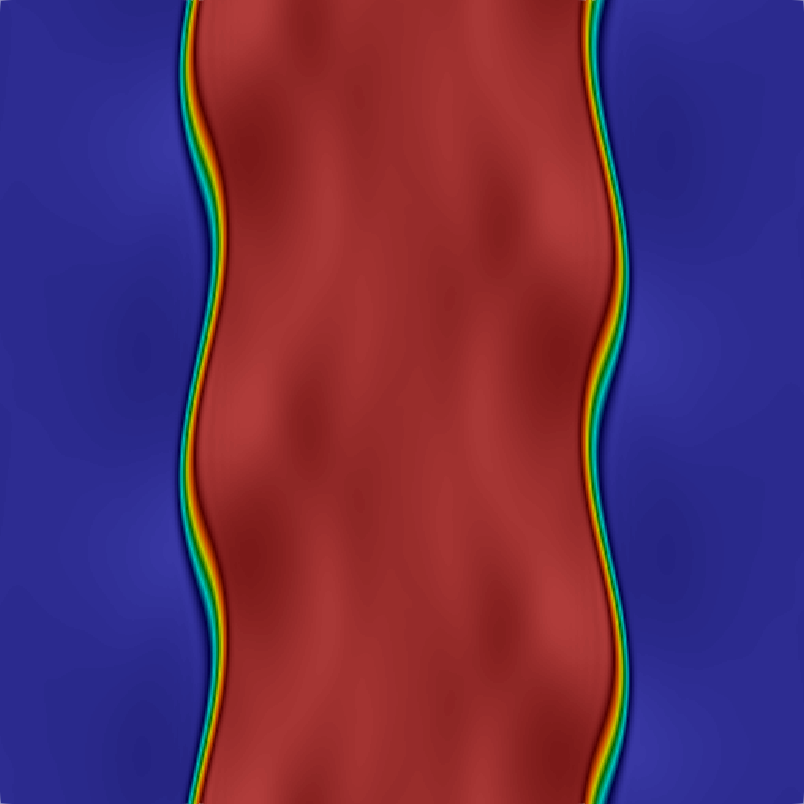
\includegraphics[scale=0.115]{data/Compressible_Euler/KH/Snapshots/density_200_307.png}\hspace{1em}
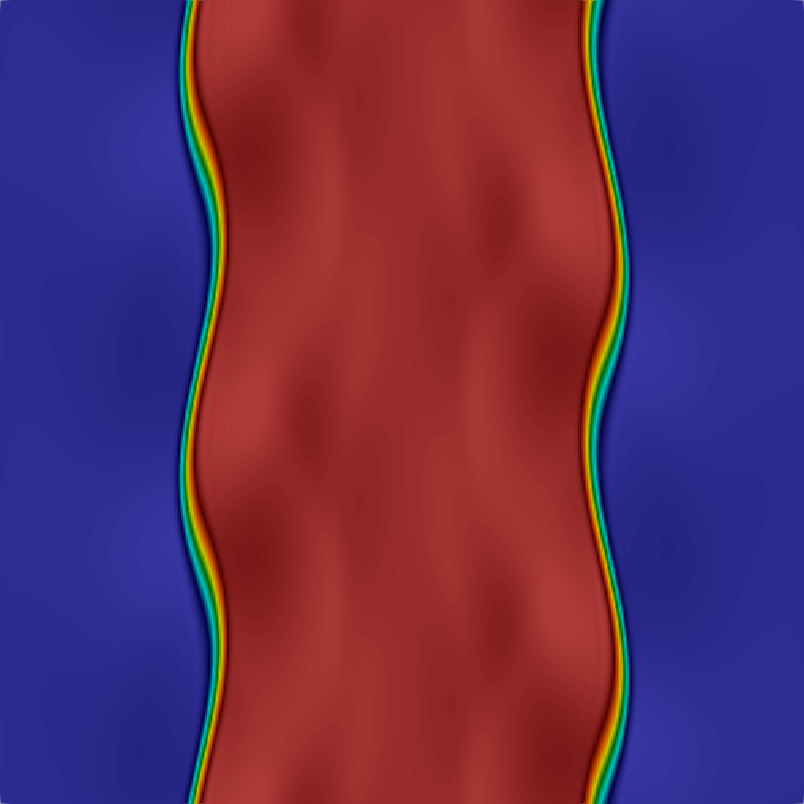
\includegraphics[scale=0.115]{data/Compressible_Euler/KH/Snapshots/density_500_307.png}\hspace{1em}
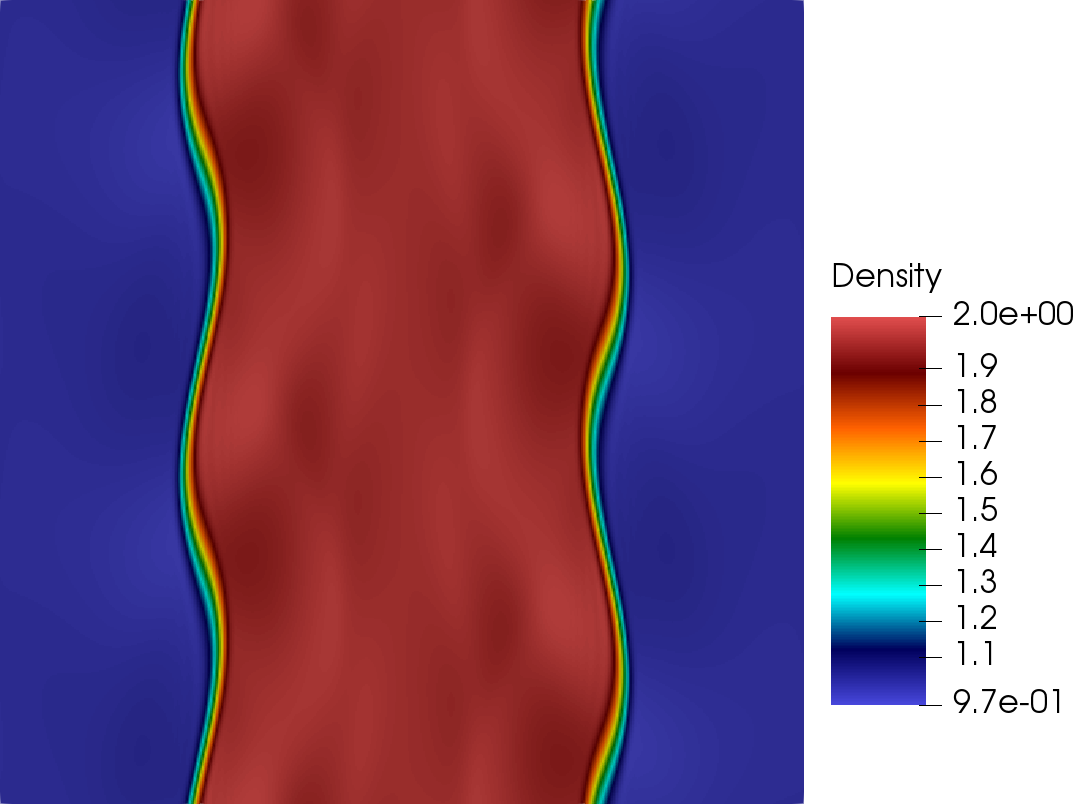
\includegraphics[scale=0.115]{data/Compressible_Euler/KH/Snapshots/density_exact_307.png}\\

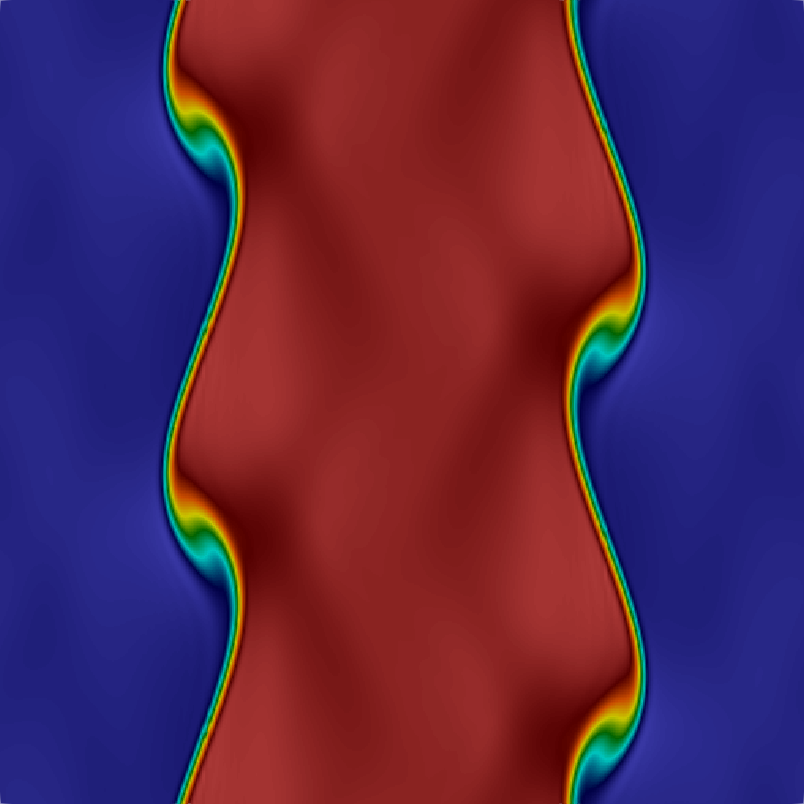
\includegraphics[scale=0.115]{data/Compressible_Euler/KH/Snapshots/density_200_461.png}\hspace{1em}
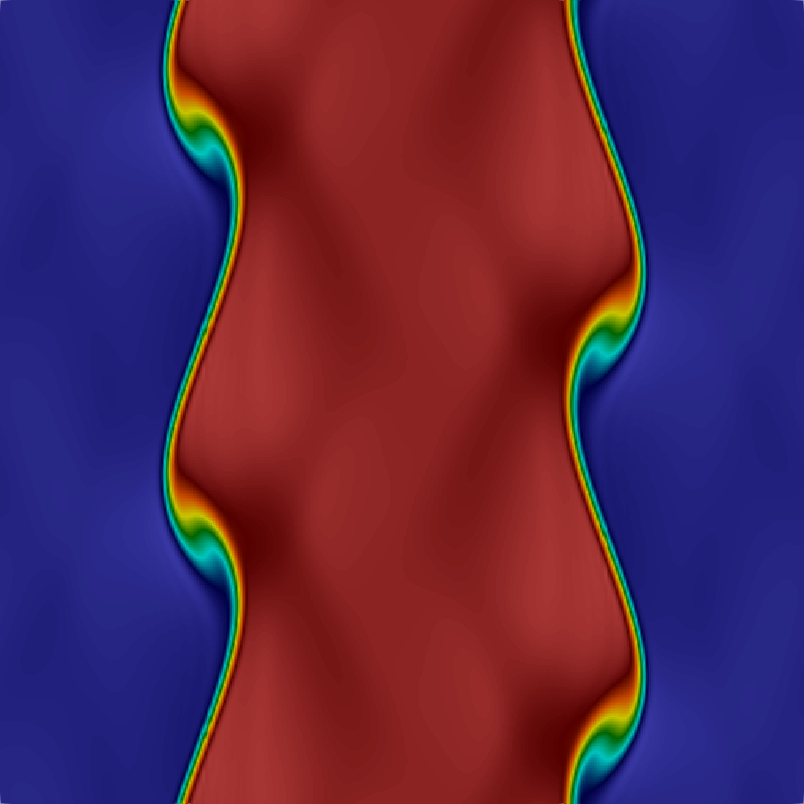
\includegraphics[scale=0.115]{data/Compressible_Euler/KH/Snapshots/density_500_461.png}\hspace{1em}
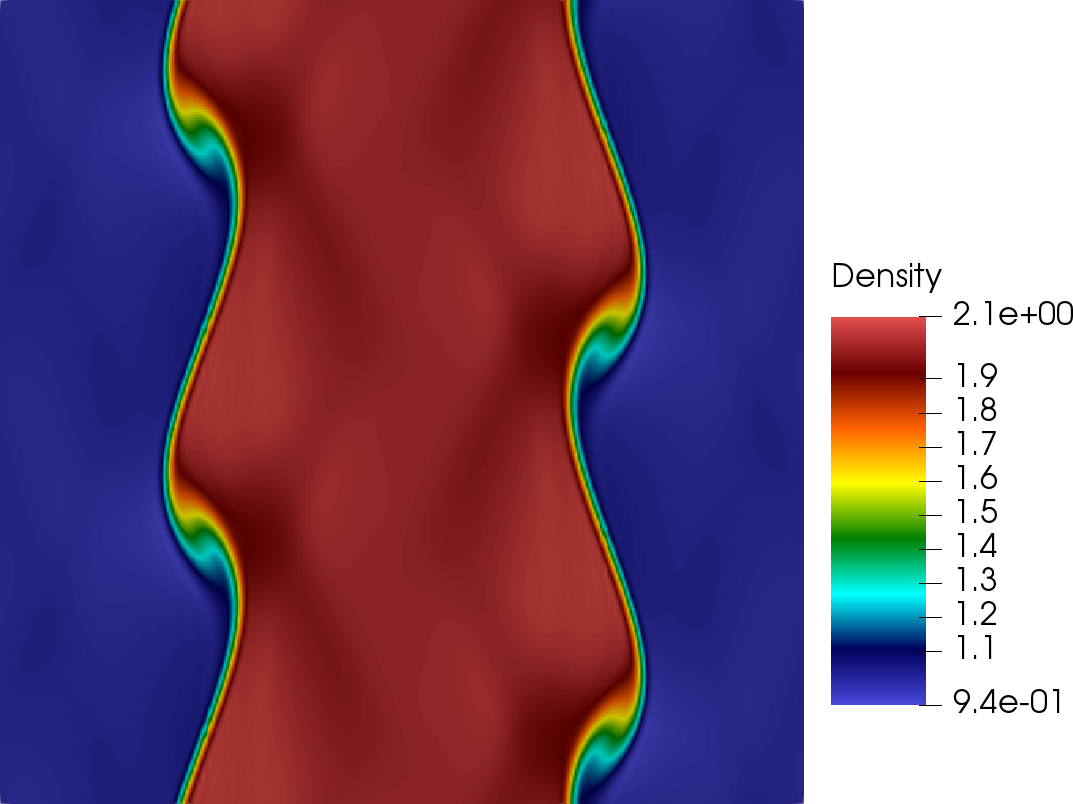
\includegraphics[scale=0.115]{data/Compressible_Euler/KH/Snapshots/density_exact_461.png}\\


\includegraphics[scale=0.115]{data/Compressible_Euler/KH/Snapshots/density_200_614.png}\hspace{1em}

\includegraphics[scale=0.115]{data/Compressible_Euler/KH/Snapshots/density_500_614.png}\hspace{1em}
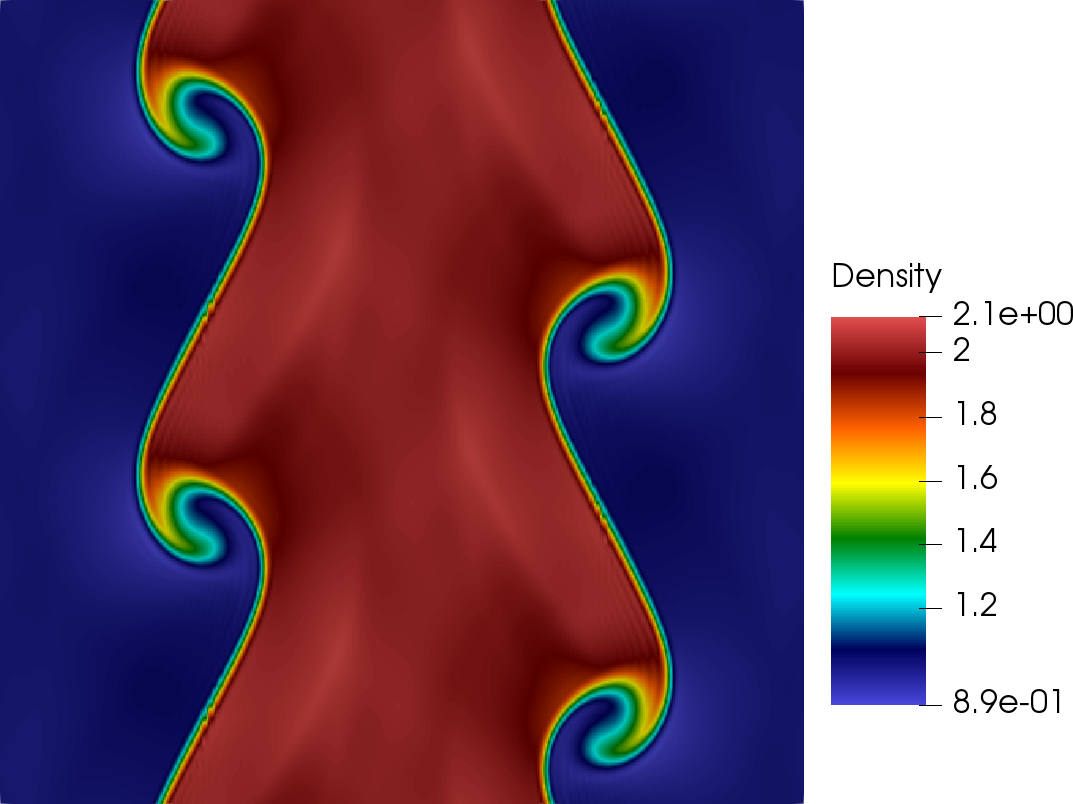
\includegraphics[scale=0.115]{data/Compressible_Euler/KH/Snapshots/density_exact_614.png}\\


\includegraphics[scale=0.115]{data/Compressible_Euler/KH/Snapshots/density_200_768.png}\hspace{1em}

\includegraphics[scale=0.115]{data/Compressible_Euler/KH/Snapshots/density_500_768.png}\hspace{1em}
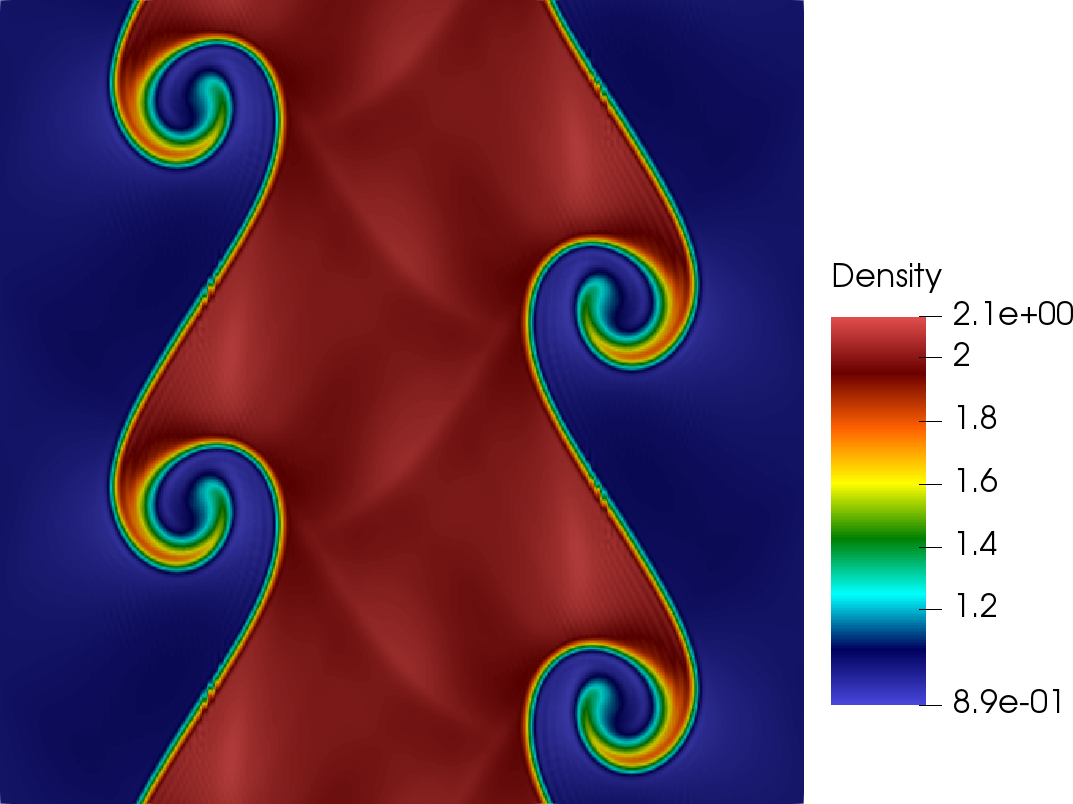
\includegraphics[scale=0.115]{data/Compressible_Euler/KH/Snapshots/density_exact_768.png}

\caption{Solutions of the Kelvin-Helmholtz problem at $t=\left\{ 0.4, 0.6, 0.8, 1 \right\}$. From left to right we have the solution of the reduced model with $k=200$, $k=500$ and the high fidelity solution.}
\label{fig:snap_solution_incompressible_Euler}
\end{figure}


\subsubsection{1D Shock problem}
%%%%%%%%%%%%%%%%%%%%%%%%%%%%%%%%%%%%%%%%%
%%%%%%%%%%%%% Singular values 1D problem %%%%%%%%%%%%%%
%%%%%%%%%%%%%%%%%%%%%%%%%%%%%%%%%%%%%%%%%
\begin{figure}
\centering
\begin{tikzpicture}[scale=0.5452]
    \begin{semilogyaxis}[ylabel = $\frac{\sigma_j}{\sum_i \sigma_i}$,
                 xlabel=Basis,
                 label style={font=\large},
                 legend style={font=\large},
                 grid=both,
                 ticks=both,
                 width=0.7\linewidth, 
                 height=0.5\linewidth,
                 minor x tick num=1,
                 minor y tick num=2,	
                 yticklabel style={/pgf/number format/.cd,fixed,precision=9},
                 scaled x ticks = true,
                 enlargelimits=false,
                 scale only axis,
                 ymin=0,
                 ymax = 2,
                 samples = 100]
                 \addplot[color=black,style=solid,style=ultra thick]  table[x = n, y = sing_values] {./data/Compressible_Euler/1D/Singular_values/sv.txt};
    \end{semilogyaxis}
\end{tikzpicture}
\caption{Singular values decay of the snapshot matrix related to POD algorithms for the 1D compressible Euler problem.}
\end{figure}

%%%%%%%%%%%%%%%%%%%%%%%%%%%%%%%%%%%%%%%%%%%%
%%%%%%%%%%%%% Mass, Total momentum & Energy %%%%%%%%%%%%%%
%%%%%%%%%%%%%%%%%%%%%%%%%%%%%%%%%%%%%%%%%%%%
\begin{figure}
  \centering
  % MASS
  \begin{subfigure}[]{0.48\linewidth}
  \begin{tikzpicture}[scale=0.55]
    \begin{axis}[ylabel = Mass,
                 xlabel=$t$,
                 label style={font=\large},
                 legend pos=north east,
                 legend entries={$k=102$ Conv,$k=201$ Conv,$k=102$ Div,$k=201$ Div,$k=102$ Skew,$k=201$ Skew},
                 legend style={font=\large},
                 grid=both,
                 ticks=both,
                 width=1.4\linewidth, 
                 height=1.0\linewidth,
                 minor x tick num=1,
                 minor y tick num=2,	
                 yticklabel style={/pgf/number format/.cd,fixed,precision=9},
                 scaled x ticks = true,
                 enlargelimits=false,
                 scale only axis,
                 ymin=0,
                 ymax = 2,
                 samples = 100]
                 \addplot[color=red,style=dashdotted,style=ultra thick]  table[x = time, y = quantity] {./data/Compressible_Euler/1D/convective_data/mass_102_1.txt};
                 \addplot[color=blue,style=dashdotted,style=ultra thick]  table[x = time, y = quantity] {./data/Compressible_Euler/1D/convective_data/mass_201_1.txt};
                 \addplot[color=red,style=dashed,style=ultra thick]  table[x = time, y = quantity] {./data/Compressible_Euler/1D/divergence_data/mass_102_1.txt};
                 \addplot[color=blue,style=dashed,style=ultra thick]  table[x = time, y = quantity] {./data/Compressible_Euler/1D/divergence_data/mass_201_1.txt};
                 \addplot[color=red,style=solid,style=ultra thick]  table[x = time, y = quantity] {./data/Compressible_Euler/1D/skew_symm_data/mass_102_1.txt};
                 \addplot[color=blue,style=solid,style=ultra thick]  table[x = time, y = quantity] {./data/Compressible_Euler/1D/skew_symm_data/mass_201_1.txt};
    \end{axis}%  
  \end{tikzpicture}
  \end{subfigure}\hfill% 
  % MASS (focus)
  \begin{subfigure}[]{0.48\linewidth}
  \begin{tikzpicture}[scale=0.55]
    \begin{axis}[xlabel=$t$,
                 label style={font=\large},
                 legend pos=south west,
                 legend entries={$k=24$ Skew,$k=102$ Skew,$k=201$ Skew},
                 legend style={font=\large},
                 grid=both,
                 ticks=both,
                 width=1.4\linewidth, 
                 height=1.0\linewidth,
                 minor x tick num=1,
                 minor y tick num=2,	
                 yticklabel style={/pgf/number format/.cd,fixed,precision=9},
                 scaled x ticks = true,
                 enlargelimits=false,
                 scale only axis,
                 ymax=0.5000001]
                 \addplot[color=black!50!green,style=solid,style=ultra thick]  table[x = time, y = quantity] {./data/Compressible_Euler/1D/skew_symm_data/mass_24_1.txt};
                 \addplot[color=red,style=solid,style=ultra thick]  table[x = time, y = quantity] {./data/Compressible_Euler/1D/skew_symm_data/mass_102_1.txt};
                 \addplot[color=blue,style=solid,style=ultra thick]  table[x = time, y = quantity] {./data/Compressible_Euler/1D/skew_symm_data/mass_201_1.txt};
    \end{axis}%  
  \end{tikzpicture}
  \end{subfigure}
 % TOTAL MOMENTUM
  \begin{subfigure}[]{0.48\linewidth}
  \begin{tikzpicture}[scale=0.55]
    \begin{axis}[ylabel = Momentum,
                 xlabel=$t$,
                 label style={font=\large},
                 legend pos=north east,
                 %legend entries={$k=24$ Div,$k=102$ Div,$k=201$ Div,$k=24$ Skew,$k=102$ Skew,$k=201$ Skew},
                 legend style={font=\large},
                 grid=both,
                 ticks=both,
                 width=1.4\linewidth, 
                 height=1.0\linewidth,
                 minor x tick num=1,
                 minor y tick num=2,	
                 yticklabel style={/pgf/number format/.cd,fixed,precision=9},
                 scaled x ticks = true,
                 enlargelimits=false,
                 scale only axis,
                 ymin=1,
                 ymax = 2,
                 samples = 100]
                 \addplot[color=red,style=dashdotted,style=ultra thick]  table[x = time, y = quantity] {./data/Compressible_Euler/1D/convective_data/momentum_102_1.txt};
                 \addplot[color=blue,style=dashdotted,style=ultra thick]  table[x = time, y = quantity] {./data/Compressible_Euler/1D/convective_data/momentum_201_1.txt};
                 \addplot[color=red,style=dashed,style=ultra thick]  table[x = time, y = quantity] {./data/Compressible_Euler/1D/divergence_data/momentum_102_1.txt};
                 \addplot[color=blue,style=dashed,style=ultra thick]  table[x = time, y = quantity] {./data/Compressible_Euler/1D/divergence_data/momentum_201_1.txt};
                 \addplot[color=red,style=solid,style=ultra thick]  table[x = time, y = quantity] {./data/Compressible_Euler/1D/skew_symm_data/momentum_102_1.txt};
                 \addplot[color=blue,style=solid,style=ultra thick]  table[x = time, y = quantity] {./data/Compressible_Euler/1D/skew_symm_data/momentum_201_1.txt};
    \end{axis}%  
  \end{tikzpicture} 
  \end{subfigure}\hfill% 
 % TOTAL MOMENTUM (focus)
  \begin{subfigure}[]{0.48\linewidth}
  \begin{tikzpicture}[scale=0.55]
    \begin{axis}[xlabel=$t$,
                 label style={font=\large},
                 legend pos=south west,
                 legend style={font=\large},
                 grid=both,
                 ticks=both,
                 width=1.4\linewidth, 
                 height=1.0\linewidth,
                 minor x tick num=1,
                 minor y tick num=2,	
                 yticklabel style={/pgf/number format/.cd,fixed,precision=9},
                 scaled x ticks = true,
                 enlargelimits=false,
                 ymax=1.04963,
                 scale only axis]
                 \addplot[color=black!50!green,style=solid,style=ultra thick]  table[x = time, y = quantity] {./data/Compressible_Euler/1D/skew_symm_data/momentum_24_1.txt};
                 \addplot[color=red,style=solid,style=ultra thick]  table[x = time, y = quantity] {./data/Compressible_Euler/1D/skew_symm_data/momentum_102_1.txt};
                 \addplot[color=blue,style=solid,style=ultra thick]  table[x = time, y = quantity] {./data/Compressible_Euler/1D/skew_symm_data/momentum_201_1.txt};
    \end{axis}%  
  \end{tikzpicture}
  \end{subfigure}
 % ENERGY
  \begin{subfigure}[]{0.48\linewidth}
  \begin{tikzpicture}[scale=0.55]
    \begin{axis}[ylabel = Energy,
                 xlabel=$t$,
                 label style={font=\large},
                 legend pos=north east,
                 %legend entries={$k=24$ Div,$k=102$ Div,$k=201$ Div,$k=24$ Skew,$k=102$ Skew,$k=201$ Skew},
                 legend style={font=\large},
                 grid=both,
                 ticks=both,
                 width=1.4\linewidth, 
                 height=1.0\linewidth,
                 minor x tick num=1,
                 minor y tick num=2,	
                 yticklabel style={/pgf/number format/.cd,fixed,precision=9},
                 scaled x ticks = true,
                 enlargelimits=false,
                 scale only axis,
                 ymin=2.5,
                 ymax = 4.5,
                 samples = 100]
                 \addplot[color=red,style=dashed,style=ultra thick]  table[x = time, y = quantity] {./data/Compressible_Euler/1D/convective_data/energy_102_1.txt};
                 \addplot[color=blue,style=dashed,style=ultra thick]  table[x = time, y = quantity] {./data/Compressible_Euler/1D/convective_data/energy_201_1.txt};                
                 \addplot[color=red,style=dashed,style=ultra thick]  table[x = time, y = quantity] {./data/Compressible_Euler/1D/divergence_data/energy_102_1.txt};
                 \addplot[color=blue,style=dashed,style=ultra thick]  table[x = time, y = quantity] {./data/Compressible_Euler/1D/divergence_data/energy_201_1.txt};
                 \addplot[color=red,style=solid,style=ultra thick]  table[x = time, y = quantity] {./data/Compressible_Euler/1D/skew_symm_data/energy_102_1.txt};
                 \addplot[color=blue,style=solid,style=ultra thick]  table[x = time, y = quantity] {./data/Compressible_Euler/1D/skew_symm_data/energy_201_1.txt};
    \end{axis}%  
  \end{tikzpicture} 
  \caption{}
  \label{conservation_1D}
  \end{subfigure}\hfill% 
 % ENERGY (focus)
  \begin{subfigure}[]{0.48\linewidth}
  \begin{tikzpicture}[scale=0.55]
    \begin{axis}[xlabel=$t$,
                 label style={font=\large},
                 legend pos=south west,
                 legend style={font=\large},
                 grid=both,
                 ticks=both,
                 width=1.4\linewidth, 
                 height=1.0\linewidth,
                 minor x tick num=1,
                 minor y tick num=2,	
                 yticklabel style={/pgf/number format/.cd,fixed,precision=9},
                 scaled x ticks = true,
                 enlargelimits=false,
                 scale only axis,
                 ymax = 2.87438]
                 \addplot[color=black!50!green,style=solid,style=ultra thick]  table[x = time, y = quantity] {./data/Compressible_Euler/1D/skew_symm_data/energy_24_1.txt};
                 \addplot[color=red,style=solid,style=ultra thick]  table[x = time, y = quantity] {./data/Compressible_Euler/1D/skew_symm_data/energy_102_1.txt};
                 \addplot[color=blue,style=solid,style=ultra thick]  table[x = time, y = quantity] {./data/Compressible_Euler/1D/skew_symm_data/energy_201_1.txt};
    \end{axis}%  
  \end{tikzpicture}
  \caption{}
  \label{conservation_1D_focus}
  \end{subfigure}
  \caption{(\protect\subref{conservation_1D})  Evolution of the three conserved quantities for the reduced solution of the compressible Euler equation (mass, total momentum and total energy).  The divergent, advective and skew-symmetric formulations have been considered and $k=102,204$ basis are used for the reduction. (\protect\subref{conservation_1D_focus}) Focus on the conserved quantity in case of stable reduction using the skew-symmetric formulation.} 
\end{figure}

%%%%%%%%%%%%%%%%%%%%%%%%%%%%%%%%%%%%%%%%%%%%
%%%%%%%%%%%%%%%% Approximation Error %%%%%%%%%%%%%%%%%
%%%%%%%%%%%%%%%%%%%%%%%%%%%%%%%%%%%%%%%%%%%%
\begin{figure}
\centering
\begin{subfigure}[]{0.48\linewidth}
  \begin{tikzpicture}[scale=0.55]
    \begin{semilogyaxis}[xlabel=$t$,
                 ylabel=$e(t)$,
                 label style={font=\large},
                 legend pos=outer north east,
                 legend style={font=\large},
                 legend entries={$k=75$,$k=126$,$k=177$,$k=225$,$k=276$,$k=327$,$k=375$,$k=426$},
                 grid=both,
                 ticks=both,
                 width=1.4\linewidth, 
                 height=1.0\linewidth,
                 minor x tick num=1,
                 minor y tick num=2,	
                 yticklabel style={/pgf/number format/.cd,fixed,precision=9},
                 scaled x ticks = true,
                 enlargelimits=false,
                 scale only axis,
                 cycle list name=exotic]
                 \addplot+[style=solid,style=ultra thick]  table[x = time, y = quantity] {./data/Compressible_Euler/1D/error/error_75.txt};  
                 \addplot+[style=solid,style=ultra thick]  table[x = time, y = quantity] {./data/Compressible_Euler/1D/error/error_126.txt};      
                 \addplot+[style=solid,style=ultra thick]  table[x = time, y = quantity] {./data/Compressible_Euler/1D/error/error_177.txt}; 
                 \addplot+[style=solid,style=ultra thick]  table[x = time, y = quantity] {./data/Compressible_Euler/1D/error/error_225.txt};      
                 \addplot+[style=solid,style=ultra thick]  table[x = time, y = quantity] {./data/Compressible_Euler/1D/error/error_276.txt};  
                 \addplot+[style=solid,style=ultra thick]  table[x = time, y = quantity] {./data/Compressible_Euler/1D/error/error_327.txt}; 
                 \addplot+[style=solid,style=ultra thick]  table[x = time, y = quantity] {./data/Compressible_Euler/1D/error/error_375.txt};      
                 \addplot+[style=solid,style=ultra thick]  table[x = time, y = quantity] {./data/Compressible_Euler/1D/error/error_426.txt};              
    \end{semilogyaxis}%  
  \end{tikzpicture}
\end{subfigure}
\caption{Evolution in time of the error  between the high fidelity solution of the 1D compressible Euler and the reduced solution for different number of basis $k$. As error measure we consider $e(t)=\sqrt{\|\mathbf{r}-\mathbf{r}^r\|^2+\|\mathbf{ur}-\mathbf{ur}^r\|^2+\|\mathbf{p}-\mathbf{p}^r\|^2}$.}
\end{figure}

%%%%%%%%%%%%%%%%%%%%%%%%%%%%%%%%%%%%%%%%%%%%
%%%%%%%%%%%%% Snapshot of pressure and density %%%%%%%%%%%%%%
%%%%%%%%%%%%%%%%%%%%%%%%%%%%%%%%%%%%%%%%%%%%
\begin{figure}
\centering
\begin{subfigure}[]{0.47\linewidth}
\begin{tikzpicture}[scale=0.58]
    \begin{axis}[xlabel=$x$,
                 ylabel=Density,
                 label style={font=\large},
                 legend pos=south west,
                 legend entries={HF,$k=24$ Div,$k=102$ Div,$k=201$ Div,$k=24$ Skew,$k=102$ Skew,$k=201$ Skew},
                 legend style={font=\large},
                 grid=both,
                 ticks=both,
                 width=1.4\linewidth, 
                 height=1.0\linewidth,
                 minor x tick num=1,
                 minor y tick num=2,	
                 yticklabel style={/pgf/number format/.cd,fixed,precision=9},
                 scaled x ticks = true,
                 enlargelimits=false,
                 scale only axis]
                 \addplot[color=black,style=solid,style=ultra thick]  table[x = time, y = energy] {./data/Compressible_Euler/1D/Snapshots/density_exact_300.txt};
                 \addplot[color=red,style=dashed,style=ultra thick]  table[x = time, y = energy] {./data/Compressible_Euler/1D/Snapshots/density_approx_unstable_24_300.txt};
                 \addplot[color=blue,style=dashed,style=ultra thick]  table[x = time, y = energy] {./data/Compressible_Euler/1D/Snapshots/density_approx_unstable_102_300.txt};
                 \addplot[color=black!50!green,style=dashed,style=ultra thick]  table[x = time, y = energy] {./data/Compressible_Euler/1D/Snapshots/density_approx_unstable_201_300.txt};
                 \addplot[color=red,style=solid,style=ultra thick]  table[x = time, y = energy] {./data/Compressible_Euler/1D/Snapshots/density_approx_24_300.txt};
                 \addplot[color=blue,style=solid,style=ultra thick]  table[x = time, y = energy] {./data/Compressible_Euler/1D/Snapshots/density_approx_102_300.txt};
                 \addplot[color=black!50!green,style=solid,style=ultra thick]  table[x = time, y = energy] {./data/Compressible_Euler/1D/Snapshots/density_approx_201_300.txt};
    \end{axis}% 
\end{tikzpicture}
\end{subfigure} 
\begin{subfigure}[]{0.47\linewidth}
\begin{tikzpicture}[scale=0.58]
    \begin{axis}[xlabel=$x$,
                 ylabel=Pressure,
                 label style={font=\large},
                 legend pos=south west,
                 %legend entries={HF,$k=24$ Div,$k=102$ Div,$k=201$ Div,$k=24$ Skew,$k=102$ Skew,$k=201$ Skew},
                 legend style={font=\large},
                 grid=both,
                 ticks=both,
                 width=1.4\linewidth, 
                 height=1.0\linewidth,
                 minor x tick num=1,
                 minor y tick num=2,	
                 yticklabel style={/pgf/number format/.cd,fixed,precision=9},
                 scaled x ticks = true,
                 enlargelimits=false,
                 scale only axis]
                 \addplot[color=black,style=solid,style=ultra thick]  table[x = time, y = energy] {./data/Compressible_Euler/1D/Snapshots/pressure_exact_300.txt};
                 \addplot[color=red,style=dashed,style=ultra thick]  table[x = time, y = energy] {./data/Compressible_Euler/1D/Snapshots/pressure_approx_unstable_24_300.txt};
                 \addplot[color=blue,style=dashed,style=ultra thick]  table[x = time, y = energy] {./data/Compressible_Euler/1D/Snapshots/pressure_approx_unstable_102_300.txt};
                 \addplot[color=black!50!green,style=dashed,style=ultra thick]  table[x = time, y = energy] {./data/Compressible_Euler/1D/Snapshots/pressure_approx_unstable_201_300.txt};
                 \addplot[color=red,style=solid,style=ultra thick]  table[x = time, y = energy] {./data/Compressible_Euler/1D/Snapshots/pressure_approx_24_300.txt};
                 \addplot[color=blue,style=solid,style=ultra thick]  table[x = time, y = energy] {./data/Compressible_Euler/1D/Snapshots/pressure_approx_102_300.txt};
                 \addplot[color=black!50!green,style=solid,style=ultra thick]  table[x = time, y = energy] {./data/Compressible_Euler/1D/Snapshots/pressure_approx_201_300.txt};
    \end{axis}% 
\end{tikzpicture}
\label{density_reduction}
\end{subfigure}

\begin{subfigure}[]{0.47\linewidth}
\begin{tikzpicture}[scale=0.58]
    \begin{axis}[xlabel=$x$,
                 ylabel=Density,
                 label style={font=\large},
                 legend pos=south west,
                 legend entries={HF,$k=24$ Div,$k=102$ Div,$k=201$ Div,$k=24$ Skew,$k=102$ Skew,$k=201$ Skew},
                 legend style={font=\large},
                 grid=both,
                 ticks=both,
                 width=1.4\linewidth, 
                 height=1.0\linewidth,
                 minor x tick num=1,
                 minor y tick num=2,	
                 yticklabel style={/pgf/number format/.cd,fixed,precision=9},
                 scaled x ticks = true,
                 enlargelimits=false,
                 scale only axis]
                 \addplot[color=black,style=solid,style=ultra thick]  table[x = time, y = energy] {./data/Compressible_Euler/1D/Snapshots/density_exact_1000.txt};
                 \addplot[color=red,style=dashed,style=ultra thick]  table[x = time, y = energy] {./data/Compressible_Euler/1D/Snapshots/density_approx_unstable_24_1000.txt};
                 \addplot[color=blue,style=dashed,style=ultra thick]  table[x = time, y = energy] {./data/Compressible_Euler/1D/Snapshots/density_approx_unstable_102_1000.txt};
                 \addplot[color=black!50!green,style=dashed,style=ultra thick]  table[x = time, y = energy] {./data/Compressible_Euler/1D/Snapshots/density_approx_unstable_201_1000.txt};
                 \addplot[color=red,style=solid,style=ultra thick]  table[x = time, y = energy] {./data/Compressible_Euler/1D/Snapshots/density_approx_24_1000.txt};
                 \addplot[color=blue,style=solid,style=ultra thick]  table[x = time, y = energy] {./data/Compressible_Euler/1D/Snapshots/density_approx_102_1000.txt};
                 \addplot[color=black!50!green,style=solid,style=ultra thick]  table[x = time, y = energy] {./data/Compressible_Euler/1D/Snapshots/density_approx_201_1000.txt};
    \end{axis}% 
\end{tikzpicture}
\end{subfigure} 
\begin{subfigure}[]{0.47\linewidth}
\begin{tikzpicture}[scale=0.58]
    \begin{axis}[xlabel=$x$,
                 ylabel=Pressure,
                 label style={font=\large},
                 legend pos=south west,
                 %legend entries={HF,$k=24$ Div,$k=102$ Div,$k=201$ Div,$k=24$ Skew,$k=102$ Skew,$k=201$ Skew},
                 legend style={font=\large},
                 grid=both,
                 ticks=both,
                 width=1.4\linewidth, 
                 height=1.0\linewidth,
                 minor x tick num=1,
                 minor y tick num=2,	
                 yticklabel style={/pgf/number format/.cd,fixed,precision=9},
                 scaled x ticks = true,
                 enlargelimits=false,
                 scale only axis]
                 \addplot[color=black,style=solid,style=ultra thick]  table[x = time, y = energy] {./data/Compressible_Euler/1D/Snapshots/pressure_exact_1000.txt};
                 \addplot[color=red,style=dashed,style=ultra thick]  table[x = time, y = energy] {./data/Compressible_Euler/1D/Snapshots/pressure_approx_unstable_24_1000.txt};
                 \addplot[color=blue,style=dashed,style=ultra thick]  table[x = time, y = energy] {./data/Compressible_Euler/1D/Snapshots/pressure_approx_unstable_102_1000.txt};
                 \addplot[color=black!50!green,style=dashed,style=ultra thick]  table[x = time, y = energy] {./data/Compressible_Euler/1D/Snapshots/pressure_approx_unstable_201_1000.txt};
                 \addplot[color=red,style=solid,style=ultra thick]  table[x = time, y = energy] {./data/Compressible_Euler/1D/Snapshots/pressure_approx_24_1000.txt};
                 \addplot[color=blue,style=solid,style=ultra thick]  table[x = time, y = energy] {./data/Compressible_Euler/1D/Snapshots/pressure_approx_102_1000.txt};
                 \addplot[color=black!50!green,style=solid,style=ultra thick]  table[x = time, y = energy] {./data/Compressible_Euler/1D/Snapshots/pressure_approx_201_1000.txt};
    \end{axis}% 
\end{tikzpicture}
\end{subfigure}

\begin{subfigure}[]{0.47\linewidth}
\begin{tikzpicture}[scale=0.58]
    \begin{axis}[xlabel=$x$,
                 ylabel=Density,
                 label style={font=\large},
                 legend pos=south west,
                 legend entries={HF,$k=24$ Div,$k=102$ Div,$k=201$ Div,$k=24$ Skew,$k=102$ Skew,$k=201$ Skew},
                 legend style={font=\large},
                 grid=both,
                 ticks=both,
                 width=1.4\linewidth, 
                 height=1.0\linewidth,
                 minor x tick num=1,
                 minor y tick num=2,	
                 yticklabel style={/pgf/number format/.cd,fixed,precision=9},
                 scaled x ticks = true,
                 enlargelimits=false,
                 scale only axis]
                 \addplot[color=black,style=solid,style=ultra thick]  table[x = time, y = energy] {./data/Compressible_Euler/1D/Snapshots/density_exact_3000.txt};
                 \addplot[color=red,style=dashed,style=ultra thick]  table[x = time, y = energy] {./data/Compressible_Euler/1D/Snapshots/density_approx_unstable_24_3000.txt};
                 \addplot[color=blue,style=dashed,style=ultra thick]  table[x = time, y = energy] {./data/Compressible_Euler/1D/Snapshots/density_approx_unstable_102_3000.txt};
                 \addplot[color=black!50!green,style=dashed,style=ultra thick]  table[x = time, y = energy] {./data/Compressible_Euler/1D/Snapshots/density_approx_unstable_201_3000.txt};
                 \addplot[color=red,style=solid,style=ultra thick]  table[x = time, y = energy] {./data/Compressible_Euler/1D/Snapshots/density_approx_24_3000.txt};
                 \addplot[color=blue,style=solid,style=ultra thick]  table[x = time, y = energy] {./data/Compressible_Euler/1D/Snapshots/density_approx_102_3000.txt};
                 \addplot[color=black!50!green,style=solid,style=ultra thick]  table[x = time, y = energy] {./data/Compressible_Euler/1D/Snapshots/density_approx_201_3000.txt};
    \end{axis}% 
\end{tikzpicture}
\caption{}
\label{density_reduction_1D}
\end{subfigure} 
\begin{subfigure}[]{0.47\linewidth}
\begin{tikzpicture}[scale=0.58]
    \begin{axis}[xlabel=$x$,
                 ylabel=Pressure,
                 label style={font=\large},
                 legend pos=south west,
                 %legend entries={HF,$k=24$ Div,$k=102$ Div,$k=201$ Div,$k=24$ Skew,$k=102$ Skew,$k=201$ Skew},
                 legend style={font=\large},
                 grid=both,
                 ticks=both,
                 width=1.4\linewidth, 
                 height=1.0\linewidth,
                 minor x tick num=1,
                 minor y tick num=2,	
                 yticklabel style={/pgf/number format/.cd,fixed,precision=9},
                 scaled x ticks = true,
                 enlargelimits=false,
                 scale only axis]
                 \addplot[color=black,style=solid,style=ultra thick]  table[x = time, y = energy] {./data/Compressible_Euler/1D/Snapshots/pressure_exact_3000.txt};
                 \addplot[color=red,style=dashed,style=ultra thick]  table[x = time, y = energy] {./data/Compressible_Euler/1D/Snapshots/pressure_approx_unstable_24_3000.txt};
                 \addplot[color=blue,style=dashed,style=ultra thick]  table[x = time, y = energy] {./data/Compressible_Euler/1D/Snapshots/pressure_approx_unstable_102_3000.txt};
                 \addplot[color=black!50!green,style=dashed,style=ultra thick]  table[x = time, y = energy] {./data/Compressible_Euler/1D/Snapshots/pressure_approx_unstable_201_3000.txt};
                 \addplot[color=red,style=solid,style=ultra thick]  table[x = time, y = energy] {./data/Compressible_Euler/1D/Snapshots/pressure_approx_24_3000.txt};
                 \addplot[color=blue,style=solid,style=ultra thick]  table[x = time, y = energy] {./data/Compressible_Euler/1D/Snapshots/pressure_approx_102_3000.txt};
                 \addplot[color=black!50!green,style=solid,style=ultra thick]  table[x = time, y = energy] {./data/Compressible_Euler/1D/Snapshots/pressure_approx_201_3000.txt};
    \end{axis}% 
\end{tikzpicture}
\caption{}
\label{pressure_reduction_1D}
\end{subfigure}
\caption{Qualitative comparison between different formulations for the reduced model in terms of density (\protect\subref{density_reduction_1D})  and pressure(\protect\subref{pressure_reduction_1D}) at $t=0.1,0.3$ and $1$s. Results for the advective formulation are not showed here because the related reduced solutions are unstable after few time steps.}
\end{figure}

\begin{figure}[h!]
\centering
\begin{subfigure}[]{0.47\linewidth}
\begin{tikzpicture}[scale=0.58]
    \begin{axis}[ylabel = e(T),
                 xlabel=Basis DEIM,
                 label style={font=\large},
                 legend pos=north east,
                 legend entries={POD+DEIM,POD},
                 legend style={font=\large},
                 grid=both,
                 ticks=both,
                 width=1.4\linewidth, 
                 height=1\linewidth,
                 minor x tick num=1,
                 minor y tick num=2,	
%                 yticklabel style={/pgf/number format/.cd,fixed,precision=9},
                 scaled x ticks = true,
                 enlargelimits=false,
                 scale only axis]
                 \addplot[color=blue,style=solid,style=ultra thick]  table[x = time, y = quantity] {./data/Compressible_Euler/1D/error_DEIM/error_DEIM.txt};      
                 \addplot[color=red,style=solid,style=ultra thick]  table[x = time, y = quantity] {./data/Compressible_Euler/1D/error_DEIM/error_POD.txt};
    \end{axis}
\end{tikzpicture}
\caption{}
\label{error_DEIM}
\end{subfigure}
\begin{subfigure}[]{0.47\linewidth}
\begin{tikzpicture}[scale=0.58]
    \begin{axis}[ylabel = Energy(T),
                 xlabel=Basis DEIM,
                 label style={font=\large},
                 legend pos=north east,
                 legend entries={POD+DEIM,POD},
                 legend style={font=\large},
                 grid=both,
                 ticks=both,
                 width=1.4\linewidth, 
                 height=1\linewidth,
                 minor x tick num=1,
                 minor y tick num=2,	
%                 yticklabel style={/pgf/number format/.cd,fixed,precision=9},
                 scaled x ticks = true,
                 enlargelimits=false,
                 scale only axis]
                 \addplot[color=blue,style=solid,style=ultra thick]  table[x = time, y = quantity] {./data/Compressible_Euler/1D/error_DEIM/error_energy_DEIM.txt};      
                 \addplot[color=red,style=solid,style=ultra thick]  table[x = time, y = quantity] {./data/Compressible_Euler/1D/error_DEIM/error_energy_POD.txt};
    \end{axis}
\end{tikzpicture}
\caption{}
\label{energy_DEIM}
\end{subfigure}
\caption{Comparison between standard POD and POD with DEIM treatment of the nonlinear term in terms of the error (\protect\subref{error_DEIM}) and the total energy (\protect\subref{energy_DEIM}).}
\label{fig:RIC2}
\end{figure}


